\documentclass{book}

\usepackage{tikz}
\usepackage[compat=1.1.0]{tikz-feynman}
\usetikzlibrary{angles, quotes}
\usetikzlibrary{calc}
\usetikzlibrary{external}
\usetikzlibrary{decorations.pathreplacing, shapes.misc}
\usetikzlibrary{decorations.markings}
\tikzexternalize[prefix=tikz/]
\tikzset{external/system call={lualatex \tikzexternalcheckshellescape -halt-on-error -interaction=batchmode -jobname "\image" "\texsource"}}
\usepackage{shellesc}


\usepackage[backend=biber, style=apa]{biblatex}  
\addbibresource{biblio.bib}


\usepackage[english]{babel}
\usepackage[a4paper]{geometry}
\usepackage{pgfplots}
\pgfplotsset{compat=1.17} 
\usepgfplotslibrary{fillbetween}

\usepackage{csquotes}
\usepackage{array}
\usepackage{multirow}
\usepackage{enumitem}
\usepackage[normalem]{ulem}
\usepackage{tabularx}
\usepackage{amsmath}
\usepackage{amssymb}
\usepackage{amsfonts}
\usepackage{physics}
\usepackage{graphicx}
\usepackage[colorlinks=true, allcolors=blue]{hyperref}
\usepackage{lineno}

\newcommand{\Ms}[0]{\textup{M}_\odot}
\newcommand{\todo}[1]{{\textcolor{gray}{\bf \large #1}}}
\newcommand{\consignes}[1]{{\textcolor{blue}{\bf \large #1}}}

\let\mcl\mathcal
\let\ov\overline
\let\ra\rightarrow

\newcolumntype{C}{>{\centering\arraybackslash}X}

\title{Second Rapport de stage de Recherche au LPNHE\\\vspace{.3em} \large Mesure de la croissance des structures avec les galaxies du DESI BGS et les supernovae de type Ia de ZTF~: vers une analyse jointe}
\author{Antoine Gilles--Lordet\\ \vspace{.1em} \small encadré par Pauline Zarrouk et Nicolas Regnault }
\date{}

\begin{document}

\maketitle

\tableofcontents

\chapter{Synthèse}

\consignes{Une synthèse d’une page (ou executive summary) présentant le problème posé et ses enjeux pour le client, les éléments clés de la démarche, les solutions apportées et les résultats obtenus, et ce, en français et en anglais}

\chapter{Introduction}

\section{Contexte}

Le modèle standard de la cosmologie, nommé $\Lambda$CDM, suppose que la gravité est décrite à toutes les échelles par la relativité générale, et que les principales contributions à la gravité viennent de la matière noire froide (\textit{Cold Dark Matter}) et l'énergie noire (sous la forme d'une constante cosmologique $\Lambda$). Ces deux inconnues sont nécessaires pour décrire l'évolution de l'Univers ainsi que la croissance des structures aux grandes échelles, et permettent à ce jour de reproduire fidèlement les observations, en particulier l'expansion accélérée de l'univers. Cependant des modèles alternatifs de gravité ont également été proposés pour expliquer cette accélération sans faire intervenir de constante cosmologique, et prédisent des évolutions temporelles différentes de celles de la relativité générale pour certaines quantités.

\subsection{Analyse du clustering des galaxies pour mesurer $f\sigma_8$}

Une de ces quantités est le facteur linéaire de croissance des structures à un redshift donné, $f(z)$, qu'il faut donc pouvoir mesurer avec précision en incluant différents effets tels que les \textbf{\textit{Redshift Space Distorsion} (RSD)} (\cite{kaiser_clustering_1987}), des distorsions liées aux transformations des coordonnées comobiles vers l'espace des redshifts. Pour mesurer la croissance des structures, la méthode la plus commune se base sur ces distorsions. Le redshift mesuré, par exemple par spectroscopie, ne contient pas uniquement le redshift cosmologique dû à l'expansion de l'univers, mais inclut également une contribution due aux vitesses particulières des galaxies par effet  Doppler.
Ce terme supplémentaire déplace les galaxies dans l'espace des redshifts par rapport à l'espace comobile, et les corrélations spatiales du champ de densité deviennent alors anisotropes : le long de la ligne de visée, les galaxies semblent plus regroupées qu'orthogonalement à la ligne de visée. A grande échelle, l'amplitude de cette anisotropie étant proportionnelle au facteur de croissance des structures $f$ et à l'amplitude des fluctuations du champ de densité, représenté communément par $\sigma_8$ (l'écart-type du champ de densité dans une sphère de rayon 8$h^{-1}$Mpc), ces analyses du clustering des galaxies contraignent le paramètre composite $f(z)\sigma_8(z)$. De nombreuses analyses des distorsions dans l'espace des redshifts ont été effectuées à l'aide de relevés spectroscopiques, tels que 6dFGRS (\cite{beutler_6df_2012}), SDSS-MGS (\cite{howlett_clustering_2015}), FastSound (\cite{okumura_subaru_2016}), SDSS-III BOSS (\cite{alam_clustering_2017}) ou SDSS-IV eBOSS (\cite{eboss_collaboration_completed_2021}). Les dernières mesures atteignent une précision de l'ordre de 10\%, et sont compatibles avec la relativité générale.

Une autre méthode pour mesurer $f\sigma_8$ est de dériver le paramètre des mesures directes des vitesses particulières des galaxies. Les vitesses particulières peuvent être mesurées directement à condition de pouvoir mesurer indépendamment les redshifts et les distances absolues des galaxies. Des mesures précises des redshifts peuvent être obtenues par spectroscopie et des estimations des distances peuvent être obtenues en utilisant les corrélations entre les distances et d'autres observables, telle que la relation de Tully-Fisher pour les galaxies spirales (corrélation entre la vitesse radiale de ses étoiles et la luminosité totale de la galaxie, \cite{tully_new_1977}) ou la méthode du Plan Fondamental (\cite{djorgovski_fundamental_1987}). Ces corrélations sont utilisables uniquement pour des galaxies à des redshifts relativement faibles ($z < 0,1$) car les incertitudes augmentent rapidement avec le redshift. Les propriétés statistiques d'un échantillon de vitesses particulières peuvent ensuite être utilisées seules ou en combinaison avec un champ de densité de galaxies.

\subsection{Analyse cosmologique avec des SN Ia}

À bas redshift, un autre moyen d'obtenir les distances vient des supernovae (SNe) de type Ia (\cite{hoyle_nucleosynthesis_1960}). Ces SNe sont des explosions thermonucléaire de naine blanche dnas un système binaire, riches en carbone et oxygène, et présentent la particularité d’avoir des conditions d'explosions très similaires les unes aux autres. Grâce à cette standardisabilité, elles constituent d'excellentes chandelles standard, et ont notamment permis la découverte de l'accélération de l'expansion de l'Univers (\cite{perlmutter_cosmology_1998, riess_observational_1998}). La réalisation d'un diagramme de Hubble\footnote{Un diagramme de Hubble est la représentation de la relation $v(d)=H(z) d$, où $v$ est la vitesse d'un objet par rapport à l'observeur et $d$ sa distance à l'observeur.} de nouvelle génération utilisant des lots encore non exploités de SN Ia des relevés \textit{Zwicky Transient Facility} (ZTF, \cite{bellm_zwicky_2018}), le SuperNovae Legacy Survey (SNLS, \cite{pritchet_snls_2004}) et Hyper Suprime-Cam Subaru Strategic Programm (HSC-SSP, \cite{miyazaki_hyper_2012,aihara_hyper_2018}) est actuellement l’objet du projet \texttt{LEMAITRE} au LPNHE. Ce projet vise à développer un nouveau pipeline d'analyse cosmologique à partir des SN Ia adapté au traitement des volumes de données attendus des prochains programmes d’observation tels que LSST (\cite{the_lsst_dark_energy_science_collaboration_lsst_2021}).

La standardisation des SN Ia est décrite par la formule de Tripp (\cite{tripp_two-parameter_1998})
\begin{equation}
\label{eq:tripp}
    M^*_{b,SN} = M_b - \alpha x_{1,SN} + \beta c_{SN} + \sigma_{int}
\end{equation}
où $M^*_{b,SN}$ est la magnitude absolue (\textit{i.e.} dans le référentiel propre) de la SN dans la bande B, $x_{1,SN}$ est le \textit{stretch} (étalement temporel) de la SN, $c_{SN}$ est la couleur (décalage spectral) de la SN, $M_b$ est la magnitude absolue moyenne à $c=0$ et $x_1=0$ dans la bande B, $\alpha$ et $\beta$ sont des coefficients valant respectivement $0.14$ et $3.15$, et $\sigma_{int}$ est la dispersion intrinsèque des SNe, elle suit une distribution Gaussienne.

Une fois la standardisation effectuée et le modèle accordé au diagramme de Hubble, les résidus au modèle donnent accès aux vitesses particulières des SNe, c’est-à-dire la vitesse des galaxies hôtes des SNe par rapport à l’expansion de l’univers (\cite{davis_effect_2011}). Cet effet est représenté en Fig. \ref{fig:residues}. Si les hôtes des SNe n’avaient pas de vitesses particulières, le redshift des SNe proviendrait uniquement de l’expansion de l’univers et elles s’aligneraient parfaitement sur le modèle. En réalité, elles sont décalées horizontalement par rapport à la ligne de base du modèle car les vitesses particulières de leurs hôtes est la source d’un effet Doppler additionnel qui modifie leur redshift~: les SNe qui se rapprochent de nous apparaissent plus bleues et celles qui s’éloignent de nous apparaissent plus rouges qu’elles ne devraient l’être. Elle fournissent donc une estimation des vitesses particulières qui peut être utilisées en combinaison avec un champ de densité de galaxies pour mener une analyse $f\sigma_8$ (\cite{boruah_bayesian_2022, stahl_peculiar-velocity_2021}). Ces analyses jointes permettent de meilleure contraintes sur $f\sigma_8$ à bas redshift que pour les analyses de RSD des galaxies (voir Fig. \ref{fig:fs8}).

\begin{figure}
    \centering
    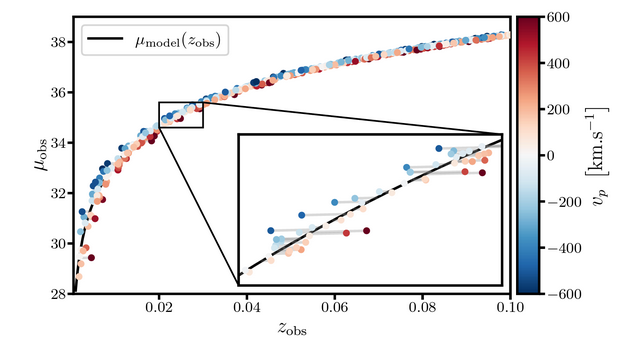
\includegraphics[width=0.8\textwidth]{figures/Residues.png}
    \caption{Diagramme de Hubble et SNe simulés. Les vitesses particulières selon la ligne de visée provoque un écart entre leur redshift cosmologique et le redshift observé, ce qui se traduit par un décalage horizontal des SNe par rapport à la ligne de base du diagramme de Hubble. Les SNe ayant une vitesse particulière positive s'éloignent de nous et nous apparaissent plus rouges, tandis que celles ayant une vitesse particulière négative nous apparaissent plus bleues. Crédit : B. Carreres}
    \label{fig:residues}
\end{figure}

\section{Objectifs}

L'objectif du stage est double~:
\begin{enumerate}
    \item Produire des échantillons simulés de SNe basés sur les positions des galaxies de la simulation Uchuu qui reproduit les données spectroscopiques du DESI BGS, ainsi que les observations de ZTF, et les utiliser pour tester le pipeline \texttt{LEMAITRE} actuellement en développement au LPNHE pour produire les diagrammes de Hubble et reconstruire la cosmologie sous-jacente des échantillons. Le pipeline étant encore en développement, je développe l'intégration des différents modules et je les teste.
    \item Comparer les résultats de ce pipeline, \textit{i.e.} les positions ainsi que les vitesses particulières reconstruites, aux données d'entrée et les utiliser pour
    	\begin{enumerate}
		\item Estimer $f \sigma_8$ à partir des vitesses particulières de SNe de ZTF et comparer ces résultats avec ceux de B. Carreres \cite{carreres_growth-rate_2023}.
		\item Produire une analyse jointe du DESI BGS et des SNe de ZTF pour quantifier le gain sur les contraintes de $f\sigma_8$.
	\end{enumerate}
\end{enumerate}

\section{Enjeux}

L'enjeu majeur de ce stage est la validation du pipeline \texttt{LEMAITRE} sur des simulations. En particulier, l'intégration faisant partie des tâches de ce stage, les différents modules n'ont été testés qu'individuellement sur des données simplifiées ou approximées. Les simulations de SNe utilisées et passées à travers tous les modules sont plus réalistes et permettront de mettre en lumière les points critiques dans l'exécution du pipeline. Ces points critiques incluent (sans être restreints à) le paramétrage des modules, des différences éventuelles de convention ou de nommage des variables utilisées, des erreurs dans les modèles, approximations ou dans leur implémentation et la caractérisation des biais potentiels.
Le fait de travailler sur des simulations permet un plus fin contrôle des conditions de test que les données réelles, et de facilement prendre en compte ou retirer différents effets.

Un second enjeu est l'estimation du gain offert par \texttt{LEMAITRE}, et plus généralement des SNe de ZTF, dans l'estimation de $f\sigma_8$. Comme évoqué précédemment, la détermination précise de ce paramètre est essentielle pour pouvoir valider ou invalider différents modèles de gravitation.



\section{Reformulation du problème dans son contexte}

\todo{Pas tout à fait sûr de ce que je dois dire}

\chapter{Approche et analyse}

\section{État de l'art}
\consignes{méthodes, raisons des choix faits, analyses menées (état de l’art)}

\subsection{Mesurer $f\sigma_8$ avec le clustering des galaxies et les SN de type Ia}
\label{sec:art}
 Plusieurs méthodes ont été développées pour extraire des mesures du taux de croissance à partir de vitesses particulières~:
 \begin{itemize}
     \item la méthode dite du maximum de vraisemblance, où les champs de vitesse (et de densité) sont supposés être tirés de distributions Gaussiennes multivariées et sur lesquels un ajustement de $f\sigma_8$ est réalisé par maximum de vraisemblance (\cite{johnson_6df_2014, huterer_testing_2017, howlett_2mtf_2017, adams_joint_2020, lai_using_2022, carreres_growth-rate_2023});
     \item l'analyse de statistiques compressées à deux points telles que la fonction de corrélation à deux points, le spectre de puissance, ou les vitesses moyennes par paire sur lesquelles $f\sigma_8$ est ajusté (\cite{nusser_velocity-density_2017, dupuy_estimation_2019, qin_redshift_2019, turner_local_2023});
     \item la comparaison entre les vitesses observées et celles reconstruites à partir du champ de densité (\cite{davis_effect_2011, carrick_cosmological_2015, boruah_cosmic_2020, said_joint_2020, stahl_peculiar-velocity_2021}). En utilisant un modèle de gravitation, on peut exprimer le champ de vitesse à partir du champ de densité et du taux de croissance des structures. Cette relation peut alors être utilisée pour obtenir $f\sigma_8$ en faisant concorder les vitesse particulières observées et celles obtenues à partir du champ de densité;
     \item l'inférence dite \textit{fieldlevel}, qui consiste à retracer l'évolution complète de l'univers à partir de conditions initiales à l'aide d'un modèle, puis à comparer le résultat obtenu aux observations des champs de densité et vitesses, et rétro-propager les erreurs jusqu'au conditions initiales (\cite{boruah_bayesian_2022, prideaux-ghee_field-based_2023}). 
\end{itemize}

Un résumé des valeurs obtenues par ces diverses analyse est représenté en Fig. \ref{fig:carreres_11}. J'utilise pour l'analyse $f\sigma_8$ la méthode décrite dans \cite{boruah_cosmic_2020,stahl_peculiar-velocity_2021}, qui est de comparer les vitesses observées reconstruites avec des SN Ia aux vitesses déduites du champ de densité. Une description plus détaillée est donnée en Annexe \ref{anx:fs8}.

\begin{figure}
    \centering
    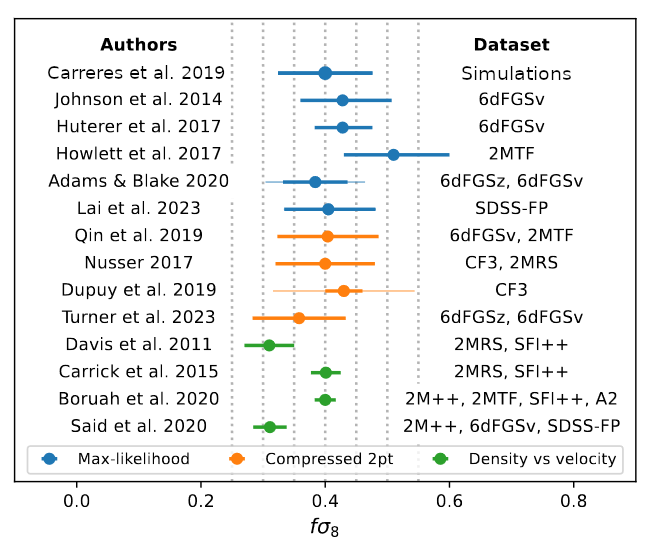
\includegraphics[width=0.7\textwidth]{figures/Carreres_fig_11.png}
    \caption{Mesures du coefficient de croissance des structures $f\sigma_8$ à partir de vitesses particulières et de catalogues de galaxies. Les barres d'erreurs en trait fin inclues les erreurs systématiques, à l'exception de Dupuy et al. 2019, pour lequel la contribution supplémentaire vient de la variance cosmique. Credit : 
    \cite{carreres_growth-rate_2023}.}
    \label{fig:carreres_11}
\end{figure}

\begin{figure}
    \centering
    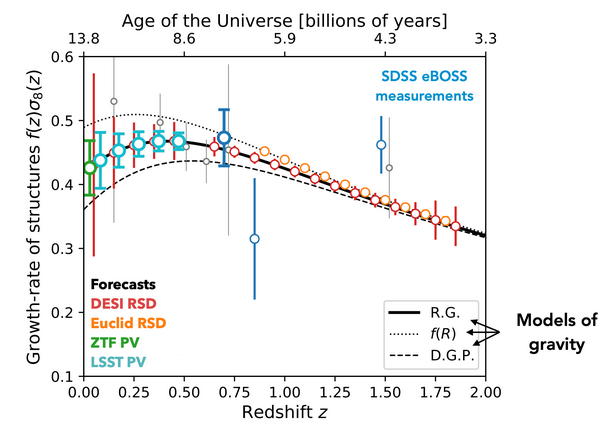
\includegraphics[width=0.8\textwidth]{figures/fs8.png}
    \caption{Prévisions des contraintes sur $f\sigma_8$ pour les relevés DESI (\cite{hahn_desi_2023}), Euclid (\cite{euclid_collaboration_euclid_2024}) et la combinaison de DESI avec des vitesses particulières de ZTF \cite{carreres_growth-rate_2023} ou LSST \cite{howlett_2mtf_2017}. Credit : J. Bautista}
    \label{fig:fs8}
\end{figure}

\section{Approche de résolution du problème}
\consignes{présentation détaillée de l’approche de résolution de problème retenue, des ressources scientifiques, techniques et humaines mises en oeuvre, de l’organisation du travail}

La méthode générale employée suit celle de \cite{carreres_growth-rate_2023} pour les simulations et reconstruction de vitesses particulières des SNe en utilisant les nouveaux modules développés pour le projet \texttt{LEMAITRE}. L'analyse $f\sigma_8$ prévue suit quand à elle celle de \cite{boruah_cosmic_2020,stahl_peculiar-velocity_2021}.

\begin{figure}
\centering
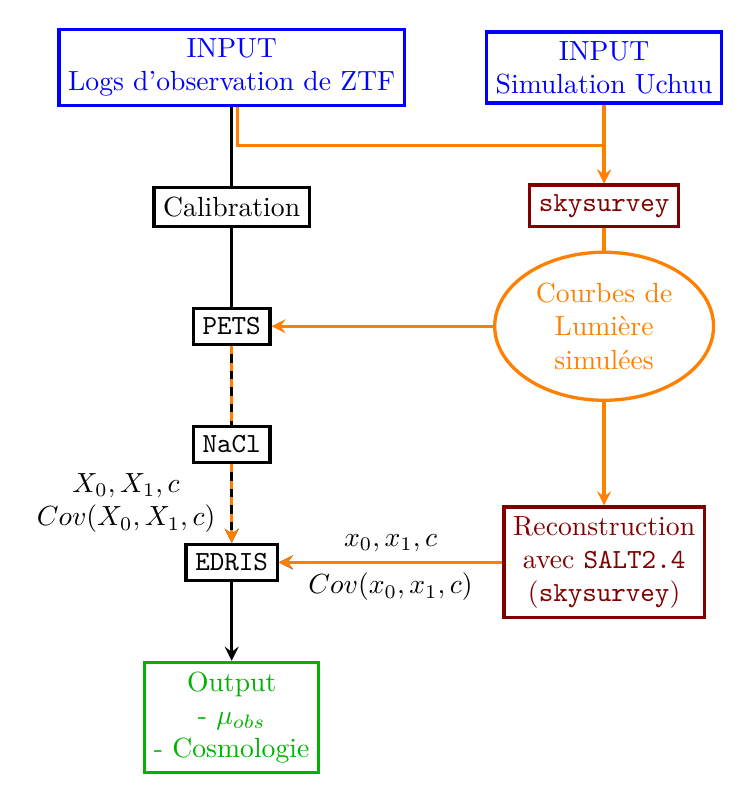
\begin{tikzpicture}[-stealth, line width=1.2pt]
	\node[rectangle, draw] (calib) at (0,0) {Calibration};
	\node[rectangle, draw, below=of calib] (pets) {\texttt{PETS}};
	\node[rectangle, draw, below=of pets] (nacl) {\texttt{NaCl}};
	\node[rectangle, draw, below=of nacl] (edris) {\texttt{EDRIS}};
	\node[rectangle, draw, below=of edris,  align=center, color=green!70!black] (out) {Output \\ - $\mu_{obs}$ \\ - Cosmologie};
	
	\node[rectangle, draw, above=of calib, color=blue, align=center] (logs) {INPUT \\ Logs d'observation de ZTF};	
	\node[rectangle, draw, right=of logs, color=blue, align=center] (uchuu) {INPUT \\ Simulation Uchuu};
	\node[rectangle, draw, below=of uchuu, red!50!black] (skys) {\texttt{skysurvey}};

	\draw (logs) -- (calib) -- (pets) -- (nacl) -- (edris) node[left=2pt, pos=0.5, align=center, black] {$X_0, X_1, c$ \\ $Cov(X_0,X_1,c)$};
	\draw (edris) -- (out);

	\begin{scope}[orange]
		\draw [dashed] (pets) -- (nacl) -- (edris);
		\path (logs) -- (skys) coordinate[pos=0.5] (A);
		\draw ([xshift=2pt]logs.south) |- (A) -| (skys);
		\draw (uchuu) -- (skys);
		\node[ellipse, draw, align=center, aspect=2] (lcsim) at (skys |- pets) {Courbes de \\ Lumière \\ simulées};
		\draw (skys) -- (lcsim) -- (pets);
	\end{scope}
	\node[rectangle, draw, align=center, red!50!black] (rec) at (lcsim |- edris) {Reconstruction \\ avec \texttt{SALT2.4} \\ (\texttt{skysurvey})};
	\draw (rec) edge node[above, align=center] {$x_0,x_1,c$} node[below, align=center] {$Cov(x_0,x_1,c)$} (edris);
	\draw[orange] (lcsim) -- (rec);
	\draw[orange] (rec) -- (edris);
\end{tikzpicture}
\caption{Chaîne d'analyse \texttt{LEMAITRE} développée au LPNHE (représentée en noire), et travail d'intégration effectué (en orange). L'étape de calibration contient en réalité plusieurs modules, mais elle n'a pas été utilisée pour ce stage car les données simulées n'incluait pas d'effets de calibration. \texttt{skysurvey} ne fait pas partie intégrante de \texttt{LEMAITRE}, il s'agit d'un sofware indépendant}
\label{fig:lemaitre_pipeline}
\end{figure}

\subsection{Génération des SN Ia et reconstruction des vitesses particulières}

Les vitesses particulières des SNe simulées ne peuvent pas être tirées aléatoirement, puisqu'elles doivent être en accord avec les structures de galaxies et les unes avec les autres. Une possibilité est de simuler la dynamique de la matière noire d'un univers via une simulation à N-corps, et de la peupler de galaxies en fonction de la distribution de densité obtenue. Cette méthode à été utilisée à partir de la simulation Uchuu (\cite{prada_desi_2023}) à 2.1 billions de particules, peuplée avec des galaxies du \textit{DESI Bright Galaxy Survey} (BGS) qui est un set complet de galaxies lumineuses ($r < 19.5$ pour le sous-échantillon \textit{Bright}) à bas redshift ($z<0.4$) (\cite{hahn_desi_2023}), pour produire un univers statistiquement fidèle au notre. Le catalogue obtenu reproduit donc à la fois le champ de densité et le champ de vitesse, à partir duquel des SNe avec vitesses particulières peuvent être tirées.

Dans un premier temps, un échantillon de SN Ia est généré selon les distributions observées des paramètres $x_0$, $x_1$, $c$ et $t_0$ (voir Table \ref{tab:snia}), et les positions et redshifts des galaxies BGS simulées dans Uchuu.

\begin{table}
    \centering
    \begin{tabular}{p{6.5cm}|p{7cm}}
         Paramètre & Distribution \\
         \hline
         Temps de maximum du flux en bande B $t_0$ & Uniforme entre le 02/03/2018 et le 01/01/2021\\
         Stretch $x_1$ & Gaussienne bimodale (\cite{nicolas_redshift_2021})\\
         Couleur $c$ &  Loi exponentielle convoluée avec une gaussienne (\cite{ginolin_ztf_2024}) \\
         Magnitude absolue $m_{abs}$ & Obtenue par la formule de Tripp\\
         Magnitude observée $m_{obs}$ & $m_{obs} = 5 \log(d_L(z)) + 25 + m_{abs}$\\
         Amplitude $x_0$ & $x_0 = 10^{0.4(m_b - m_{obs})}$
    \end{tabular}
    \caption{Distributions des paramètres pour le tirage des SN Ia}
    \label{tab:snia}
\end{table}

Seules les galaxies à redshift $z<0.06$ sont utilisées afin de s'affranchir du biais de Malmquist (voir notamment \cite{carreres_growth-rate_2023} ou \cite{boyd_accounting_2024}). Ce biais observationnel vient du fait que les télescopes ont une magnitude limite d'observation, au-delà de laquelle les SNe ne sont plus détectées. Or, à un redshift donné, les SNe couvrent une plage de magnitude du fait de la dispersion due aux paramètres de standardisations, à la dispersion intrinsèque et aux vitesses particulières. Ainsi, à haut redshift, les SNe les moins brillantes ne sont pas observées, ce qui biaiserait une estimation des paramètres cosmologique. ZTF est considéré complet jusqu'à $z=0.6$, ce qui signifie que l'impacte du biais de Malmquist en dessous de ce redshift est négligeable.

La période du 02/03/2018 au 01/01/2021 utilisée pour le tirage du temps de maximum correspond à la plage temporelle de la DR2.5 de ZTF qui sera exploitée par \texttt{LEMAITRE}. Cette restriction sert à la fois à avoir un volume de donné proche de celui que devra traiter le pipeline \texttt{LEMAITRE} pour estimer sa rapidité, et à pouvoir quantifier le gain qui pourrait être obtenu sur $f\sigma_8$ avec des réelles. Le taux d'explosions de SN Ia est pris égal à $2,35 .10^4$Gpc$^{-3}$ (\cite{perley_zwicky_2020}).
Pour le calcul de la magnitude observée, $d_L(z)$ représente la distance de luminosité, qui est calculée à l'aide d'un modèle $\Lambda$CDM contraint par les données de Planck 2015 (\cite{planck_collaboration_planck_2016}) pour correspondre au modèle cosmologique utilisé pour générer la simulation Uchuu.

Une fois les paramètres tirés, des points de données d'observations photométriques et spectroscopiques sont générés en utilisant le modèle de SNe \texttt{SALT2.4} (\cite{guy_salt2_2007, rigault_ztf_2024}) et les logs d'observations de ZTF. Ce modèle consiste en trois fonctions $M_0(p, \lambda)$, $M_1(p, \lambda)$ et $CL(\lambda)$ de manière à décrire les flux émis par les SNe dans leurs référentiels propres par~:
\begin{equation}
    F(SN, p, \lambda) = x_0 \times \qty[M_0(p, \lambda) + x_1 M_1(p, \lambda)] \times \exp[c CL(\lambda)]
\end{equation}
où $p$, nommé phase, est le temps dans le référentiel de la SN depuis la date du maximum de luminosité dans la bande B, $\lambda$ est la longueur d'onde dans le référentiel de la SN, $x_0$ est l'amplitude du flux, et $x_1$ et $c$ sont les paramètres de standardisations de stretch et couleur.

Une fois les observations simulées, le set de donné obtenu est passé à travers les différents modules du pipeline \texttt{LEMAITRE}~:
\begin{enumerate}
    \item Le module PETS (Preprocessing and sElection of a Training Sample) effectue une première sélection en éliminant les points de photométrie ainsi que les SNe mal mesurés. Il donne également une première évaluation des paramètre de standardisation des SNe, qui sert de point de départ pour NaCl, voir Annexe \ref{anx:pets}.
    \item Le module NaCl (Nouvel algorithme de Courbe de lumière) ajuste un modèle type \texttt{SALT2.4} aux SNe et réévalue les paramètres de standardisations. Il fournit également la matrice de covariance des paramètres des différentes SN et des paramètres des modèles ajustés, voir Annexe \ref{anx:nacl}.
    \item Le module EDRIS (Estimateur de Distance pour les Relevés Incomplets de Supernovae) utilise les paramètres de standardisations et leur matrice de covariance pour ajuster un modèle cosmologique sur les points de données et évaluer les paramètres $\alpha$ et $\beta$ du modèle de Tripp (eq. \ref{eq:tripp}), voir Annexe \ref{anx:edris}.
\end{enumerate}

Avec les résultats d'EDRIS, on peut remonter aux modules de distances
\begin{equation}
    \mu = m_b - M_b^*
\end{equation}
où $m_b$ est la magnitude maximale dans la bande B.
Comme les modules de distances ne dépendent que du redshift via le modèle cosmologique, en théorie $\mu = \mu(z)$ et tout les points devraient s'aligner sur le modèle (à une dispersion Gaussienne introduite par $\sigma_{int}$ près). En réalité comme mentionné en section \ref{sec:art}, les vitesses particulières ont pour effet de décaler les redshifts observés. Les points de données sont décalés horizontalement par rapport à la courbe théorique de $\mu(z)$ (voir Fig. \ref{fig:residues} et \ref{fig:edris_fit}).

\begin{figure}
    \centering
    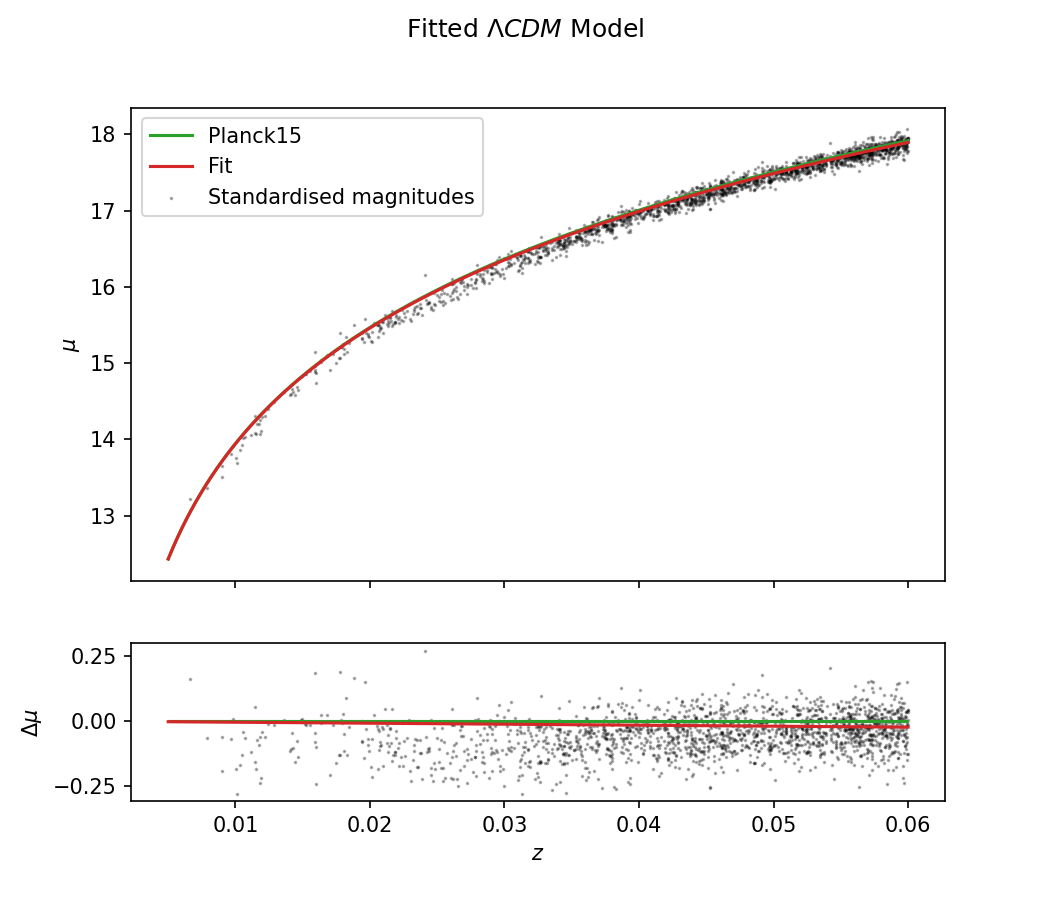
\includegraphics[width=0.8\linewidth]{figures/edris_model_fit.png}
    \caption{Modèle et standardisation ajustés par EDRIS}
    \label{fig:edris_fit}
\end{figure}

On peut alors inverser cette courbe pour obtenir une relation $z(\mu)$, c'est-à-dire obtenir le redshift auquel correspond un module de distance, puis remonter aux vitesses particulières en utilisant~:
\begin{equation}
    v_p = c (z_{obs} - z(\mu))
\end{equation}
avec $c$ la vitesse de la lumière.

\section{Résultats intermédiaires et finaux visés}
\consignes{présentation des résultats intermédiaires et finaux visés}

\todo{Générer des SNe avec des vitesses particulières tirées d'Uchuu avec skysurvey}

\todo{Les reconstruire avec SALT2.4}

\todo{ou traiter avec PETS puis reconstruction NaCl}

\todo{Utiliser EDRIS sur les résultats SALT2.4 et NaCl}

\todo{Obtenir les VP}

\todo{Obtenir une grille de densité adaptée pour l'analyse fs8}

\todo{Réaliser l'analyse fs8}



\section{Difficultés rencontrées}
\consignes{exposé des difficultés rencontrées et de la façon dont elles ont été surmontées}

La principale difficulté que j'ai rencontré a été de suivre le développement des différents modules de \texttt{LEMAITRE} tout en les utilisant et en remplissant mes tâches. Puisque l'intégration des modules n'était pas encore réalisée, j'ai pu identifier différents problèmes qui y étaient lié tels que des différences de convention ou de notation pour des variables. Mes tests ont également permis de révéler certains comportements anormaux des modules lors de leurs utilisation sur des données réalistes (par exemple des erreurs liées à des paramètres sortant des plages de définition du modèle dans NaCl), et de mettre en lumière des étapes de filtrages des données entre les modules afin d'assurer leurs bons fonctionnements. Cela a nécessité de faire des points pour discuter de l'avancement des modules en plus des points hebdomadaires prévus avec les autres membres de l'équipe, afin de remonter et résoudre les problèmes rencontrés, et être à jour sur l'utilisation des modules.

Une autre difficulté notable a été la compréhension fine du domaine et des tâches, afin de proposer une analyse correcte et robuste. J'ai parfois eu du mal à différencier certains concepts et outils, mais avec des explications et l'aide de mes encadrants et des autres chercheurs de l'équipe, j'ai pu surmonter cette difficulté.

\todo{Les saletés de float32 de skysurvey}

\todo{problèmes d'évaluation des bandes dans bbf}

\todo{PETS et la détection des minimums locaux trop proches/mauvaises estimations du Tmax}

\todo{variances négatives pour edris ou NaCl du à un mauvais point initial/une mauvaise convergence (importance du premier fit pour NaCl}

\todo{Extension du modèle pour NaCl pour bien intégrer les bandes.}

\todo{valeurs de la régularisation et des contraintes NaCl}

\todo{Problème sur la condition d'arrêt du tncg d'edris}

\todo{Importance des cuts sur les incertitudes pour edris (et lien avec la densité de la matrice)}

\todo{Biais sur $\beta$ lorsque les couleurs sont trop élevées}


\todo{Les accords pour les données DESI/ZTF/BORG}


\section{Gestion des risques réalisée}
\consignes{gestion des risques réalisée}

\todo{Tout commentaire ou idée à mettre dans cette partie est la bienvenue}

\chapter{Résultats}
\consignes{présentation détaillée des résultats effectivement obtenus en les reliant au problème qui était à traiter et mettant en exergue :
\begin{itemize}
\item la validité des résultats par rapport au problème
\item le caractère innovant / neuf des résultats
\item l’utilité des résultats, l’usage effectif qui sera fait du travail de l’élève ingénieur
\item la mise en exergue des limites du travail et des suites à donner à ce travail
\item la quantification et/ou qualification de la valeur ajoutée
\end{itemize}}


\section{Validation de LEMAITRE sur simulations}
\todo{Génération des SNe avec des vitesses particulières tirées d'Uchuu avec skysurvey}

\todo{Les reconstruire avec SALT2.4}

\todo{ou traiter avec PETS puis reconstruction NaCl}

\todo{Utiliser EDRIS sur les résultats SALT2.4 et NaCl}



\section{Extraction des vitesses particulières}

Les vitesses particulières ainsi obtenues sont représentées en Fig. \ref{fig:vp}. Les vitesses reconstruites sont en très bon accord avec les vitesses injectées : l'erreur moyenne n'est que de $54$km.s$^{-1}$ et l'écart type de l'erreur commise est de 410km.s$^{-1}$, ce qui est faible sachant que les vitesses particulières valent en moyenne $\sim 200$km.s$^{-1}$ et présentent une dispersion de $\sim 300$km.s$^{-1}$.   L'effet de la dispersion intrinsèque sur l'estimation des vitesses particulières est particulièrement visible à haut redshift, car la contribution des vitesses particulières au redshift observé est alors plus faible, et le module de distance évolue plus lentement avec le redshift.

\begin{figure}
    \centering
    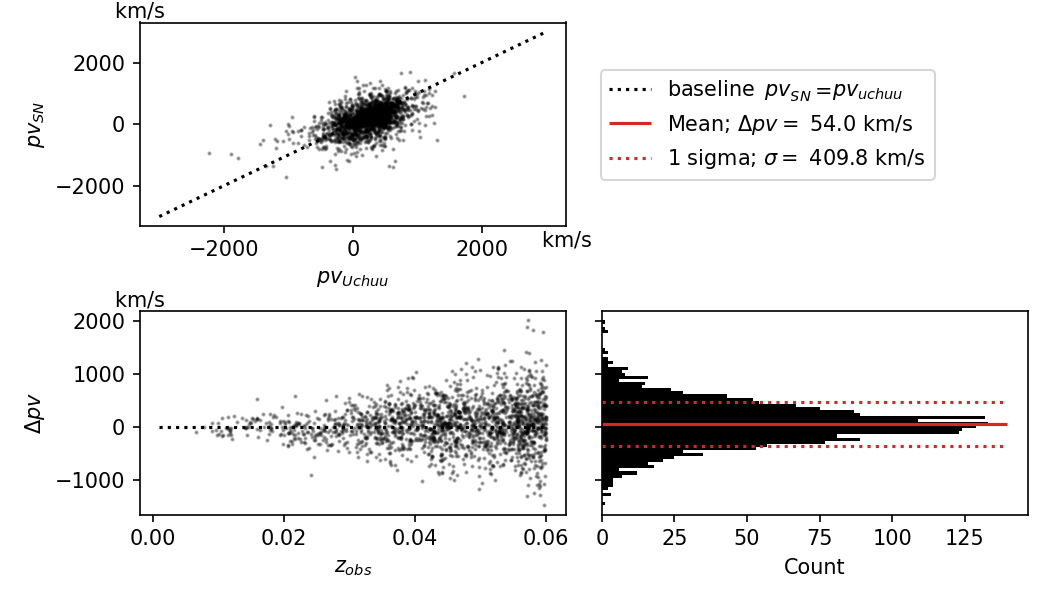
\includegraphics[width=0.8\textwidth]{figures/edris_vp_uchuu_vs_edris.png}
    \caption{Comparaison entre les vitesses particulières injectées (dénommée $pv_{Uchuu}$) et les vitesses particulières reconstruites ($pv_{edris}$).}
    \label{fig:vp}
\end{figure}


\chapter{Travail futur}
\consignes{prolongements possibles du travail de stage : exposé de ce qu’il reste éventuellement à faire pour que les résultats soient complètement obtenus, et de la façon dont le travail pourra être poursuivi par l’entreprise dans le futur}

\todo{FS8}

\chapter{Bilan personnel}
\consignes{bilan des principaux apprentissages professionnels et leur mise en perspective pour le futur professionnel}

\todo{TODO}

\chapter{Enjeux éthiques}
\consignes{prise de recul sur les enjeux d’ordre éthique}

\todo{}

\appendix
\chapter{Annexes}
\pagenumbering{roman}

\section{Fonctionnement des modules}

\subsection{\texttt{PETS}}
\label{anx:pets}

PETS a pour but de sélectionner les SN qui sont suffisamment bien échantillonnées pour l'entraînement du modèle par NaCl.
Le fonctionnement de PETS est découpé en 3 étapes, tous utilisant le modèle \texttt{SALT2.4} déjà entraîné~:
\begin{enumerate}
\item Une sélection des points de donnés utilisables.
\item La réalisation d'une grille de temps de maximums et des fits associés à chacun de ces temps
\item La sélection des SNe
\end{enumerate}

La sélection des points de données est effectuée en rejetant itérativement les points de données à plus de 3$\sigma$ du fit \texttt{SALT2.4}. Ensuite, en partant du $t_{max, 0}$ d'un fit complet des points restants, une grille de temps de maximum est réalisé. Elle contient 150 points dans les intervalles $[t_{max, 0} - 20 ; t_{max, 0} - 5]$ et $[t_{max, 0} +5; t_{max, 0} + 20]$ et 1000 points dans l'intervalle $[t_{max, 0} - 5 ; t_{max, 0} + 5]$. Le modèle est alors fitté sur les données en fixant le temps de maximum à un de ces points, puis PETS analyse la courbe $\chi^2(t_{max})$ afin de garder ou rejeter la SN. Une SN est gardée si~:
\begin{enumerate}
\item $\chi^2(t_{max})$ présente un minimum global à $t_{min}$, qui n'est pas aux bords de l'intervalle $[t_{max,0} - 20 ; t_{max, 0} + 20]$
\item L'incertitude sur $t_{min}$ est inférieure à 1 jour.
\item L'écart entre les incertitudes positives et négatives à 3$\sigma$ est inferieur à $0.3$, ce qui caractérise la symétrie de $\chi^2(t_{max})$ autour de $t_{min}$.
\item $\chi^2(t_{max})$ ne présente pas d'autres minimums à 8$\sigma$ de ce minimum global, \textit{i.e.} il n'y a pas d'autres minimums proches susceptibles de coincer le fit de NaCl.
\item Les valeurs de $x_1$ et $c$ fittées sont respectivement inférieures à 4 et 2, ce qui impose que le fit ne décrit pas une SN extrêmement distordue (bien qu'elle soit toujours décrite par le modèle).
\end{enumerate}

Une version mise à jour de PETS utilisant un modèle NaCl pré-entraîné à la place de \texttt{SALT2.4} est en cours de développement, mais je ne l'ai pas utilisée.


\subsection{\texttt{NaCl}}
\label{anx:nacl}

\subsubsection{Modélisation des SNe}

\texttt{NaCl} consiste en une implémentation d'un modèle type \texttt{SALT}, avec quelques améliorations. Tout comme \texttt{SALT}, le flux émis par les SNe dans leurs référentiels propres est modélisé par une surface spectrale $\mcl S(\lambda, p)$, où $\lambda$ est la longueur d'onde d'émission dans le référentiel de la SN, $p$, la phase, est le temps depuis le maximum d'émission en bande B.
De cette surface de flux, on peut déduire dans notre référentiel à la fois le flux photométrique, c'est-à-dire le flux observé dans un filtre de bande passante $T(\lambda)$ à une date donnée, et les spectres émis en redshiftant cette surface~:
\begin{gather}
	\phi_{phot} = X_0 \frac{1}{1+z} \int \mcl S\qty(\frac{\lambda}{1+z}, p) \frac{\lambda}{hc} T(lambda) \dd{\lambda} \label{eq:phot}\\
	\phi_{spec}  = X_0 \frac{1}{1+z} \mcl S(\lambda, p) \label{eq:spec}
\end{gather}
où $X_0 = \Phi_B \frac{(10\text{pc}^2}{d_L(z)^2}$ est l'amplitude, avec $\Phi_B$ la luminosité maximale en bande B normalisée pour une SN à 10 pc, et $d_L(z)$ est la distance de luminosité. Toute l'information sur la cosmologie est donc encodée dans $X_0$ via la distance de luminosité.
Pour réduire le temps de calcul, l'équation \ref{eq:phot} est ré-exprimée en intégrant dans le référentiel de la SN, ce qui équivaut à blueshifter les filtres plutôt que de redshifter la surface spectrale~:
\begin{equation}
	\phi_{phot} = X_0 (1+z) \int \mcl S(\lambda, p) \frac{\lambda}{hc} T((1+z)\lambda) \dd{\lambda}
\end{equation}

La surface spectrale est décrite de la même manière que pour \texttt{SALT2.4} avec la paramétrisation par SN suivante
\begin{equation}
    \mcl S (p, \lambda) = \qty[M_0(p, \lambda) + X_1 M_1(p, \lambda)] \times \exp[0..4 c CL(\lambda)]
\end{equation}
où , et $X_1$ et $c$ sont les paramètres de stretch et couleurs propre à la SN considérée.

\subsubsection{Différences entre NaCl et SALT2.4}

Les différences entre \texttt{NaCl} et \texttt{SALT2.4} ne sont pas liés au modèle de SNe lui-même, mais à des choix dans les paramètres ajustés lors de l'entraînement~:
\begin{itemize}
\item Le temps du maximum $t_{max}$ n'est plus déterminé avant entraînement et fixé, mais est laissé comme paramètre libre. Autrement dit, les points de donnés dans l'espace des phases $(\lambda, p)$ sont susceptibles de bouger selon $p$, puisque décaler la date de maximum revient à décaler d'autant tous les points de mesures.
\item La calibration des filtres est intégrée dans le modèle ce qui permet d'estimer directement son impact sur les paramètres reconstruits, plutôt que d'entraîner le modèle sur différents lots avec des calibrations variables.
\item En conséquence de la différence précédente, le modèle d'erreur, c'est à dire l'incertitude du modèle sur les valeurs de flux, est également ajusté lors de l'entraînement plutôt qu'estimé a posteriori.
\end{itemize}
Le lecteur attentif aura noté que les amplitudes et stretch de SALT était notées avec des minuscules $x_0$ et $x_1$, tandis que celles de NaCl sont notées avec des majuscules $X_0$ et $X_1$. Cette différence est intentionnelle, puisque du fait des différences dans l'entraînement, rien ne garantit que ces paramètres sont exactement les mêmes, ce qui n'est d'ailleurs pas le cas dans les faits (\textcolor{red}{cf Résultats}).


\subsubsection{Contraintes}

En conséquence de ces choix, les contraintes imposées sur les modèles diffèrent de celles utilisées pour entraîner \texttt{SALT2.4}. Une des idées fondamentales de ces contraintes est que $M_0$ doit décrire la SN moyenne, et que tous les termes autour ne doivent être que des corrections. Cela ce traduit par exemple dans la normalisation des modèles, dégénérée avec $X_0$, en imposant
\begin{gather}
	\int M_0(p=0,\lambda) \frac{\lambda}{hc} B(\lambda) \dd{\lambda} = 1\\
	\int M_0(p=0,\lambda) \frac{\lambda}{hc} B(\lambda) \dd{\lambda} = 0
\end{gather}
De même, les couleurs et stretchs sont contraints pour être de moyenne nulle, par
\begin{gather}
	\sum_{i=1}^{N_{SN}} c_i = 0\\
	\sum_{i=1}^{N_{SN}} X_{1,i} = 0\\
\end{gather}
À cela s'ajoute une dégénérescence liée aux normalisations des $X_1$ relativement à $M_1$, qui est levée en imposant une contrainte sur la variance des $X_1$
\begin{gather}
	\frac{1}{N_{SN}} \sum_{i=1}^{N_{SN}} (X_{1,i} - \ev{X_1})^2 = 1
\end{gather}

La variabilité du temps de maximum introduit également une dégénérescence avec les modèles $M_0$ et $M_1$. Cette dégénérescence est brisée en imposant aux modèles de présenter un maximum en bande B à $p=0$~:
\begin{gather}
	\eval{\dv{p} \int M_0(p,\lambda) \frac{\lambda}{hc} B(\lambda) \dd{\lambda}}_{p=0} = 0\\
	\eval{\dv{p} \int M_1(p,\lambda) \frac{\lambda}{hc} B(\lambda) \dd{\lambda}}_{p=0} = 0
\end{gather}

 \subsubsection{Entraînement}

L'entraînement a lieu en 3 étapes après initialisation des modèles $M_0$ et $M_1$ sur les modèles de \texttt{SALT2.4}. Une première estimation des paramètres de chaque SN $(x_0, x_1, c, t_{max})$ est réalisée à modèles et modèle d'erreur fixés. Ensuite, les paramètres des SNe sont fixés aux valeurs obtenues, et seul le modèle d'erreur est laissé libre et ajusté. Pour finir, tous les paramètres sont relâchés et le modèle est ajusté en même temps que les paramètres des SNe et le modèle d'erreur. C'est lors de cette dernière étape que les contraintes décrites précédemment sont effectivement appliquées au modèle, puisque \texttt{SALT2.4} intégrait d'autres contraintes.

Ce choix vient du fait qu'un entraînement sur tous les paramètres seraient trop coûteux et qu'il pourrait se bloquer plus facilement dans un minimum local.


\subsection{\texttt{EDRIS}}
\label{anx:edris}

Le module \texttt{EDRIS} réalise un diagramme de Hubble en ajustant un modèle cosmologique aux modules de distances de SNe.

\section{Méthode de l'analyse jointe $f\sigma_8$}
\label{anx:fs8}

Comme mentionné précédemment, l'analyse $f\sigma_8$ se base sur la méthode de comparaison entre les vitesses particulières et celles obtenues à partir du champ de densité, plus précisément sur la méthodologie de \cite{stahl_peculiar-velocity_2021}.

La relation entre le champ de vitesse et le contraste de densité des galaxies $\delta_g = \frac{\rho_g}{\ov{\rho_g}} - 1$ est donné par~:
\begin{equation}
    \vb v (\vb r) = \frac{H_0 \mcl B}{4 \pi} \int_0^{R_{max}} \dd[3]{\vb r'} \delta_g(\vb r') \frac{\vb r' - \vb r}{\abs{\vb r' - \vb r}} + \vb V_{ext}
\end{equation}
où $\mcl B =\frac{f}{b}$, avec $b$ le biais entre le contraste de densité des galaxies et celui de la matière noire ($\delta_g = b \delta_{DM}$), $R_{max}$ est la distance maximale couverte par le catalogue, et $\vb V_{ext}$ est le flux cohérent causé par des structures à l'extérieur du catalogue.

Les vitesses obtenues à partir du champ de densité sont alors ajustées sur celles des vitesses particulières issues des SN à partir d'une méthode \textit{Forward Likelihood}. Les paramètres $\mcl B$ et $\vb V_{ext}$ ainsi que d'autres paramètres de nuisance liés aux observations $\vb \Theta$ (notamment les paramètres du modèle de Tripp $\alpha$, $\beta$, $M_b$ et $\sigma_{int}$, voir Eq. \ref{eq:tripp}) sont reliés aux paramètres observables des SN $(\vb x_i)$ via la probabilité conditionnelle $\mcl P(\mcl B, \vb V_{ext}, \vb \Theta | \vb x_i)$, qui peut être exprimée à l'aide du théorème de Bayes
\begin{equation}
    \mcl P(\mcl B, \vb V_{ext}, \vb \Theta | \vb x_i) \propto \mcl P(\vb x_i|\mcl B, \vb V_{ext}, \vb \Theta) \mcl P(\mcl B, \vb V_{ext}, \vb \Theta)
\end{equation}
Les priors sur les paramètres de nuisance du modèle de Tripp sont non restrictifs, ils imposent simplement $\alpha, \beta > 0$ et $M < 0$, tandis que $\sigma_{int}$ est log-normale avec un pic à $0.15$ mag.

Pour corriger d'éventuelles inhomogénéités selon différentes lignes de visées, on doit introduire de plus une distribution radiale
\begin{equation}
    \mcl P(\vb r|\vb \Theta) = \frac{1}{\mcl N(\vb \Theta)} r^2 \exp{- \frac{\qty[\mu(\vb r) - \mu(\vb\Theta)]^2}{2 \sigma_\mu^2(\vb \Theta)}} \qty[1 + \delta_g(\vb r)]
\end{equation}
où $\vb r$ est un vecteur comobile pointant sur la sphère célèste, $\mcl N(\vb \Theta)$ est un coefficient de normalisation, $\mu$ est le module de distance, et $\sigma_\mu$ est l'erreur sur le module de distance causée par la dispersion intrinsèque des SNe. On obtient alors la vraisemblance suivante
\begin{equation}
    \mcl P(\vb x_i|\mcl B, \vb V_{ext}, \vb \Theta) = \int_0^{R_{max}} \dd{r} \mcl P (\vb x_i|\vb r, \mcl B, \vb V_{ext}, \vb \Theta) \mcl P(\vb r|\vb \Theta)
\end{equation}
avec
\begin{equation}
     \mcl P (\vb x_i|\vb r, \mcl B, \vb V_{ext}, \vb \Theta) = \frac{1}{\sqrt{2 \pi \sigma_\nu^2}} \exp{-\frac{\qty[c z_{obs} - cz_{pred}(\vb r, \mcl B, \vb V_{ext})]^2}{2\sigma_\nu^2}}
\end{equation}
$z_{obs}$ est le redshift observé de la SN, et $z_{pred}$ est la prédiction de ce redshift à partir du redshift cosmologique et des vitesses reconstruites grâce à
\begin{equation}
    1 + z_{pred}(\vb r, \mcl B, \vb V_{ext}) = (1 + z_{cosmo}(\vb r)) \qty[1 + \frac{1}{c} (\mcl B \vb v(r) + \vb V_{ext}) \cdot \vu r]
\end{equation}
$\sigma_\nu$ peut-être soit ajusté avec les autres paramètres de nuisance comme dans \cite{stahl_peculiar-velocity_2021}, auquel cas il suit une dispersion gaussienne, soit fixé comme dans \cite{boruah_cosmic_2020}.

Finalement, la log-vraisemblance s'écrit
\begin{equation}
    \mcl L = \ln \mcl P(\mcl B, \vb V_{ext}, \vb \Theta) + \sum_i P(\vb x_i|\mcl B, \vb V_{ext}, \vb \Theta)
\end{equation}
Cette vraisemblance est alors explorée avec une Chaîne de Markov Monte Carlo, et produit des résultats comme ceux de \cite{stahl_peculiar-velocity_2021} représentés en Fig. \ref{fig:stahl}, qui sont en très bon accord avec d'autres analyses $f\sigma_8$ et ont une meilleure précision que les analyses $f\sigma_8$ utilisant seulement les RSD.

\begin{figure}
    \centering
    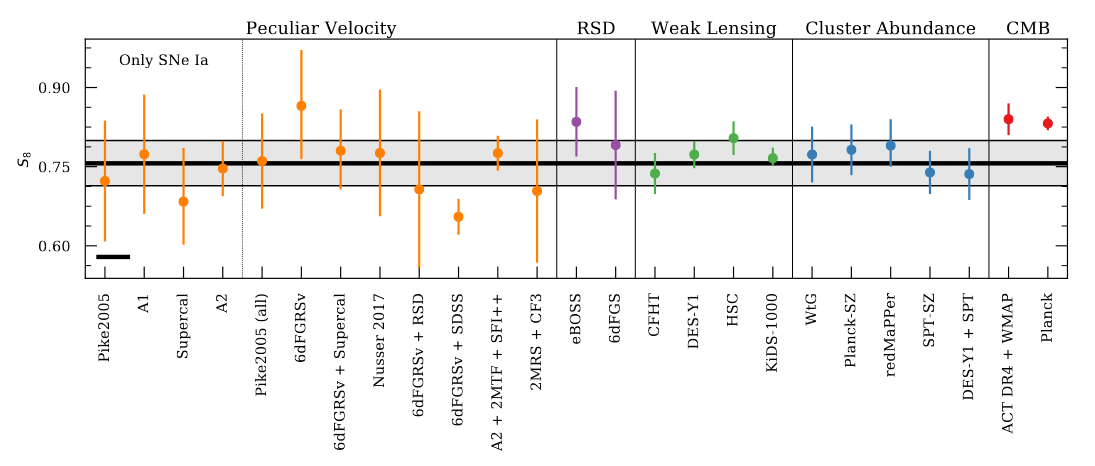
\includegraphics[width=0.8\textwidth]{figures/Stahl_fig_6.png}
    \caption{Paramètre $S_8 = f \sigma_8/(0.3)^{0.55}$ reconstruit par diverses méthodes. Les lignes noires représentent la valeur et l'incertitude de la valeur reconstruite par \cite{stahl_peculiar-velocity_2021}. Crédit : B. Stahl}
    \label{fig:stahl}
\end{figure}


\printbibliography

\end{document}
